\documentclass[11pt,letterpaper]{article}
\usepackage{fullpage}

\usepackage[english]{babel}
\usepackage[utf8]{inputenc}
\usepackage{amsmath}
\usepackage{graphicx}
\usepackage[hidelinks]{hyperref}
\usepackage{float}
\usepackage{amsfonts}
\usepackage{algorithm,algpseudocode}
\usepackage{pdfpages}
             
\graphicspath{{../results}}

\begin{document} 

\title{Competing Bandits Overview}
\maketitle

\section*{Simulation Details}

Considered $K = 3$, $Memory = 100$ (unless otherwise noted) \\
\textbf{The Bandit priors that were considered}:
\begin{itemize}
\item Uniform: Draw the mean rewards for the arms from [0.25, 0.75]
\item ``HeavyTail": We took the mean rewards to be randomly drawn from Beta($\alpha=0.6,\beta=0.6$). With this distribution it was likely to have arms that were at the extremes (close to 1 and close to 0) but also some of the arms with intermediate value means.
\item Needle-in-haystack
\begin{enumerate}
\item High - 2 arms with mean 0.50, 1 arm with mean 0.70 (+ 0.20)
\end{enumerate}
\end{itemize}
\textbf{Algorithms considered}:
\begin{enumerate}
\item ThompsonSampling with priors of $Beta(1, 1)$ for every arm.
\item DynamicGreedy with priors of $Beta(1, 1)$ for every arm
\item Bayesian Dynamic $\epsilon$-greedy with priors of $Beta(1, 1)$ for every arm and $\epsilon=0.05$
\end{enumerate}
\textbf{Agent Algorithms considered}:
\begin{enumerate}
\item HardMax
\item HardMaxWithRandom ($\epsilon = 0.05$)
\item SoftMax ($\alpha = 30$)
\end{enumerate}
\textbf{Memory Sizes}
\begin{enumerate}
\item 100
\end{enumerate}
\pagebreak
\textbf{Competing Bandits Simulation Procedure}
\begin{algorithm}
\begin{algorithmic}[1]
\For{Each prior $p$}
\State Generate true distribution from $p$ (except for needle-in-haystack, just use $p$ itself)
\State Generate $T \times K$ realizations for the arms 
	\For{Each agent algorithm $agent alg$}
		\For{Each principal algorithm pair $principalalg1$, $principalalg2$}
			\For{$N$ simulations}
				
				\State Give the agents $k$ observations from each principal
				\State Give principal 2 $X$ free observations (the agents also get these observations)
				\State Run simulation for T periods
			\EndFor
		\EndFor
	\EndFor
\EndFor
\end{algorithmic}
\end{algorithm}

\section*{Preliminary Calibration}

First, let's look at the preliminary simulation results on the instances we considered. In these simulations we simply run the selected bandit algorithm on the selected prior (no competition).  What is plotted here is the reputation score for a memory size of $100$ for each of the priors and each of the algorithms (recall that reputation score is the average of the last 100 observations):

\includegraphics[scale=0.5]{"../results/preliminary_figures/Reputation Trajectory for Needle In Haystack High 3 arms"} \\
\includegraphics[scale=0.5]{"../results/preliminary_figures/Reputation Trajectory for Uniform 3 arms"} \\
\includegraphics[scale=0.5]{"../results/preliminary_figures/Reputation Trajectory for Heavy Tail 3 arms"}

One thing which may be problematic with these plots is that for Heavy Tail and Uniform the means for the instances are randomly drawn for each simulation but these plots just take averages over all of the simulations.

Some additional preliminary calibration plots. These plots show the \% of simulations over $N=200$ that identified the best arm over time (based on looking at the posterior distributions at a given time): \\
\includegraphics[scale=0.5]{"needle_in_haystack_best_arm_ident"} \\
\includegraphics[scale=0.5]{"heavy_tail_best_arm_ident"} \\
\includegraphics[scale=0.5]{"uniform_best_arm_identification"} 


\section*{Simultaneous Entry}

The first set of results we will consider are $X = 0$ and $k = 5$ so that there is simultaneous entry. Recall to read the tables: \\
\begin{enumerate}
\item In bold is the average market share for principal 1 and with a 95\% confidence interval
\item The var term is the variance of the market shares
\item The ``share" line means the \% of simulations that ended up with one principal getting more than 90\% of the market.
\end{enumerate}


\textbf{Question of Interest}: What algorithms should win under different agent response models? \\
\textbf{Overall Conjecture}: For the agent response functions with randomness (HMR and SoftMax), the algorithm performance in the later rounds of the single agent case should dictate which algorithm does better in the long-run in the competing bandits game. For the agent response functions without randomness (HM), the algorithm that does better in the very short-run of the single agent case should do better in the long-run in the competing bandits game. \\
\textbf{Conjecture}: HardMaxWithRandom and SoftMax should eventually lead to the better algorithm winning as long as, on the instance we are considering there is a gap in the long-term reward of the better algorithms. \\
\textbf{Why?} Looking at the preliminary calibration plots, since there is some randomness in the choice rule of the agents, each principal should always be getting some free observations (our parameters such as the $\alpha$ in SoftMax and $\epsilon$ in HardMaxWithRandom tune how many expected observations a principal should get for a fixed $T$).  Let's fix attention on the case of ThompsonSampling vs Bayesian/Dynamic Greedy. Looking at each of the preliminary plots we see that ThompsonSampling beats Dynamic / Bayesian Greedy for sufficiently large $T$. Thus, if we calibrate the time horizon long enough so that the principal playing Thompson Sampling should, in expectation, get sufficiently many samples to be on the part of the curve where learning is almost done then it should be able to accumulate a higher reputation score (by having better arm selection than DynamicGreedy) and eventually get more of the market. \\

\textbf{Conjecture}: Under HardMax, the early rounds should dictate almost everything since we suppose the algorithms start with little initial information and thus the difference between the algorithms should not make much of a difference. Since the rewards are randomly drawn, lucky early round draws may dictate the course of the game. Thus a conjecture is that the mean market share will be 50/50.

The first conjecture seems to be confirmed in the simulations. Using the calibration from above ($\epsilon = 0.05$ for HMR and $\alpha = 30$ for SoftMax). However, the HardMax results require some more validation. First, we look at the results for low $T$ (1000) but high $N$ (1200). Then we extend the time horizon, but look at lower $N$. One annoying note, it is hard to compare SoftMax across these next two simulations since in the first $\alpha = 10$ and the in the second $\alpha = 30$

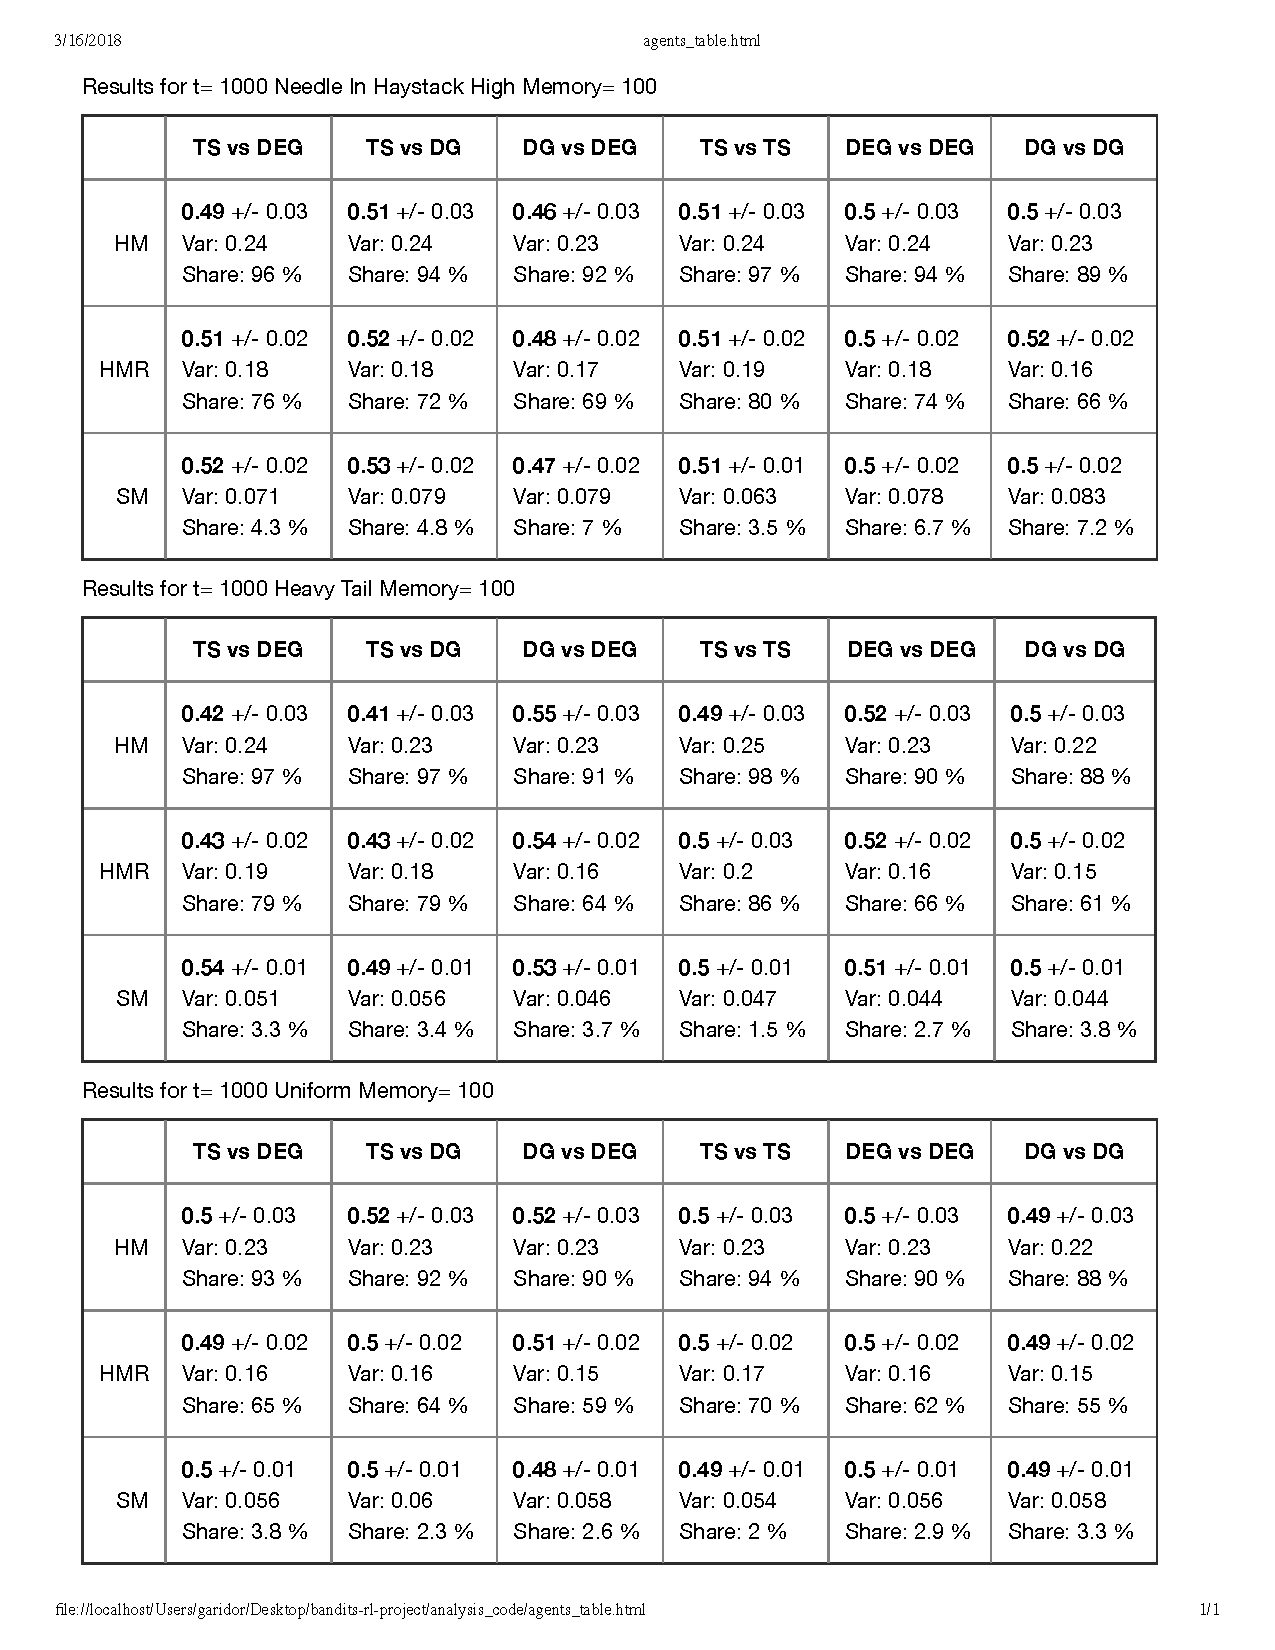
\includepdf[pages={-}]{low_time_high_num_sim}

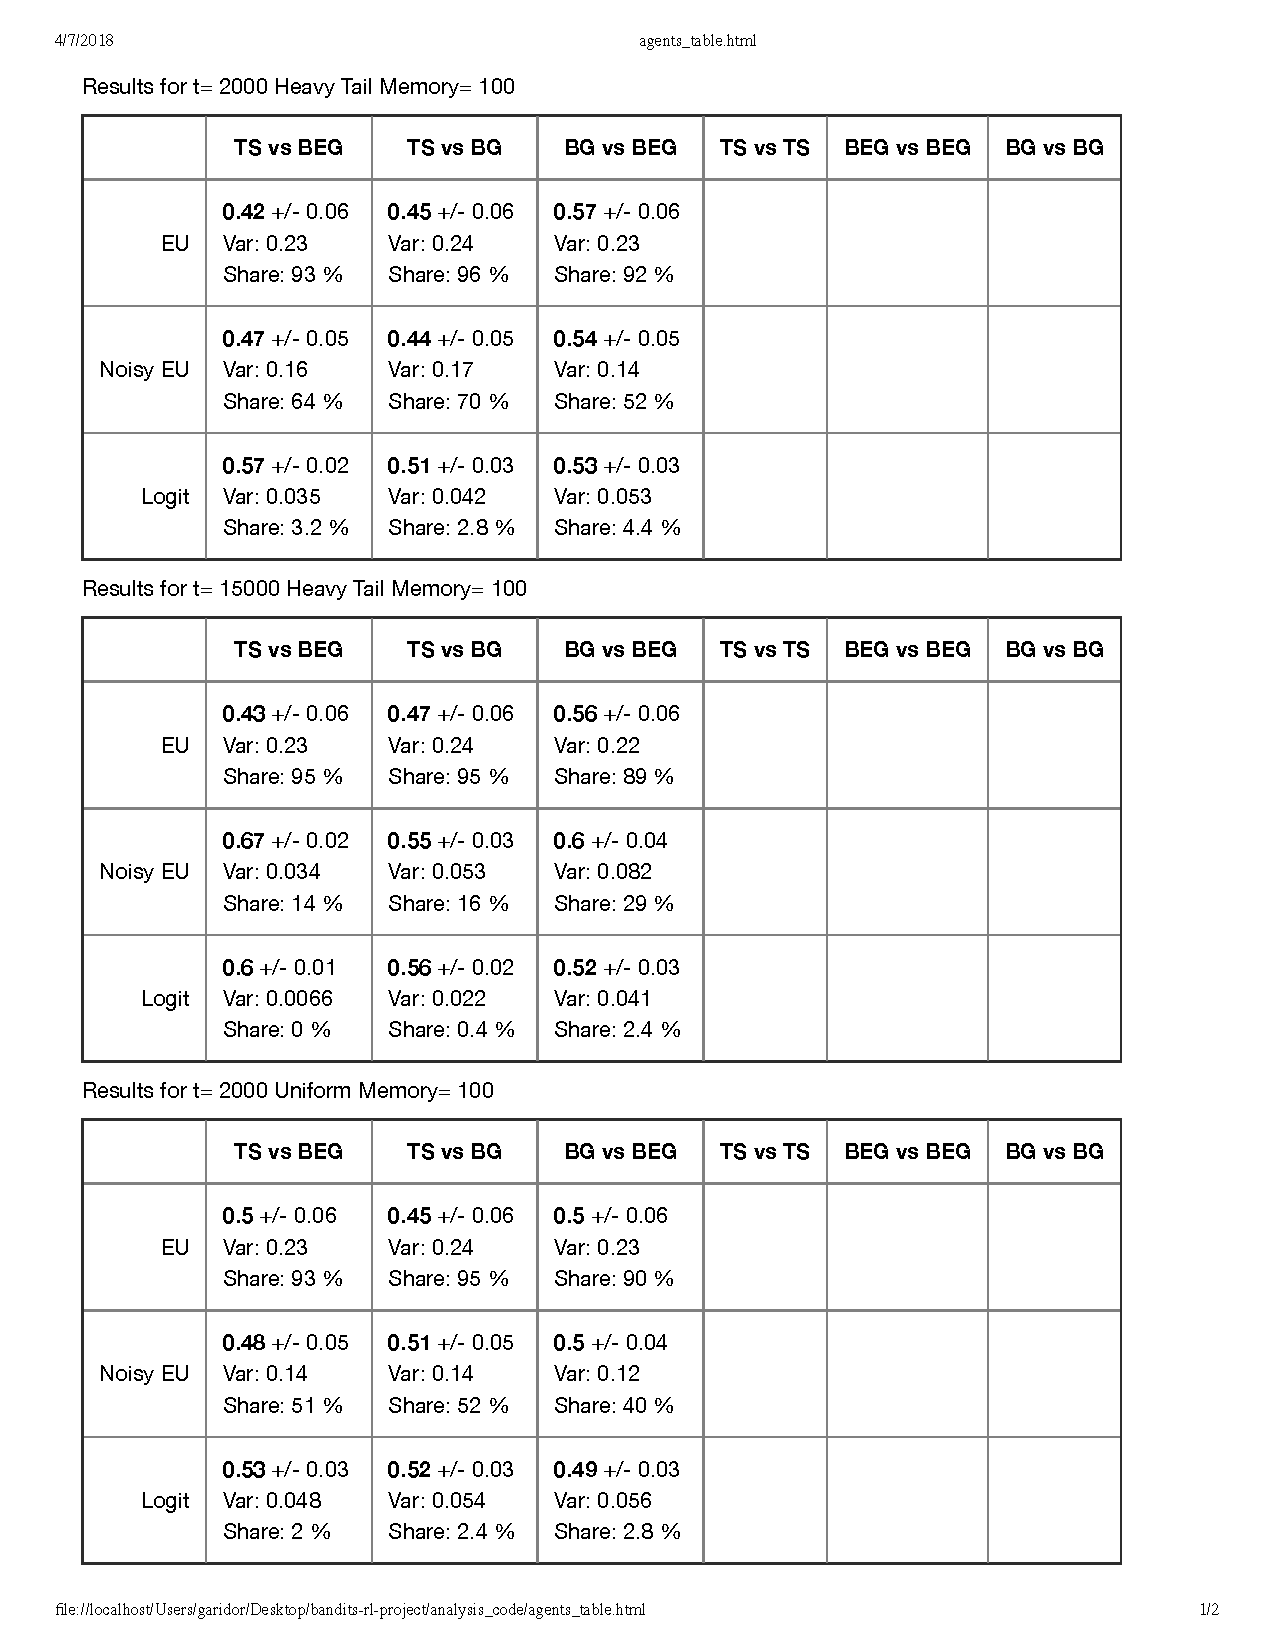
\includepdf[pages={-}]{tournament_results}

The conjecture for HMR and SM seems to be consistent with the data generated from the simulation (the one exception seems to be HeavyTail for BG vs BEG - more on this later). However, what is going on with HardMax appears confusing. To get some more evidence for the original conjecture, we re-run simulations but track market share over time. In most cases, we get evidence of this and the vast majority of market shares over time look as follows:

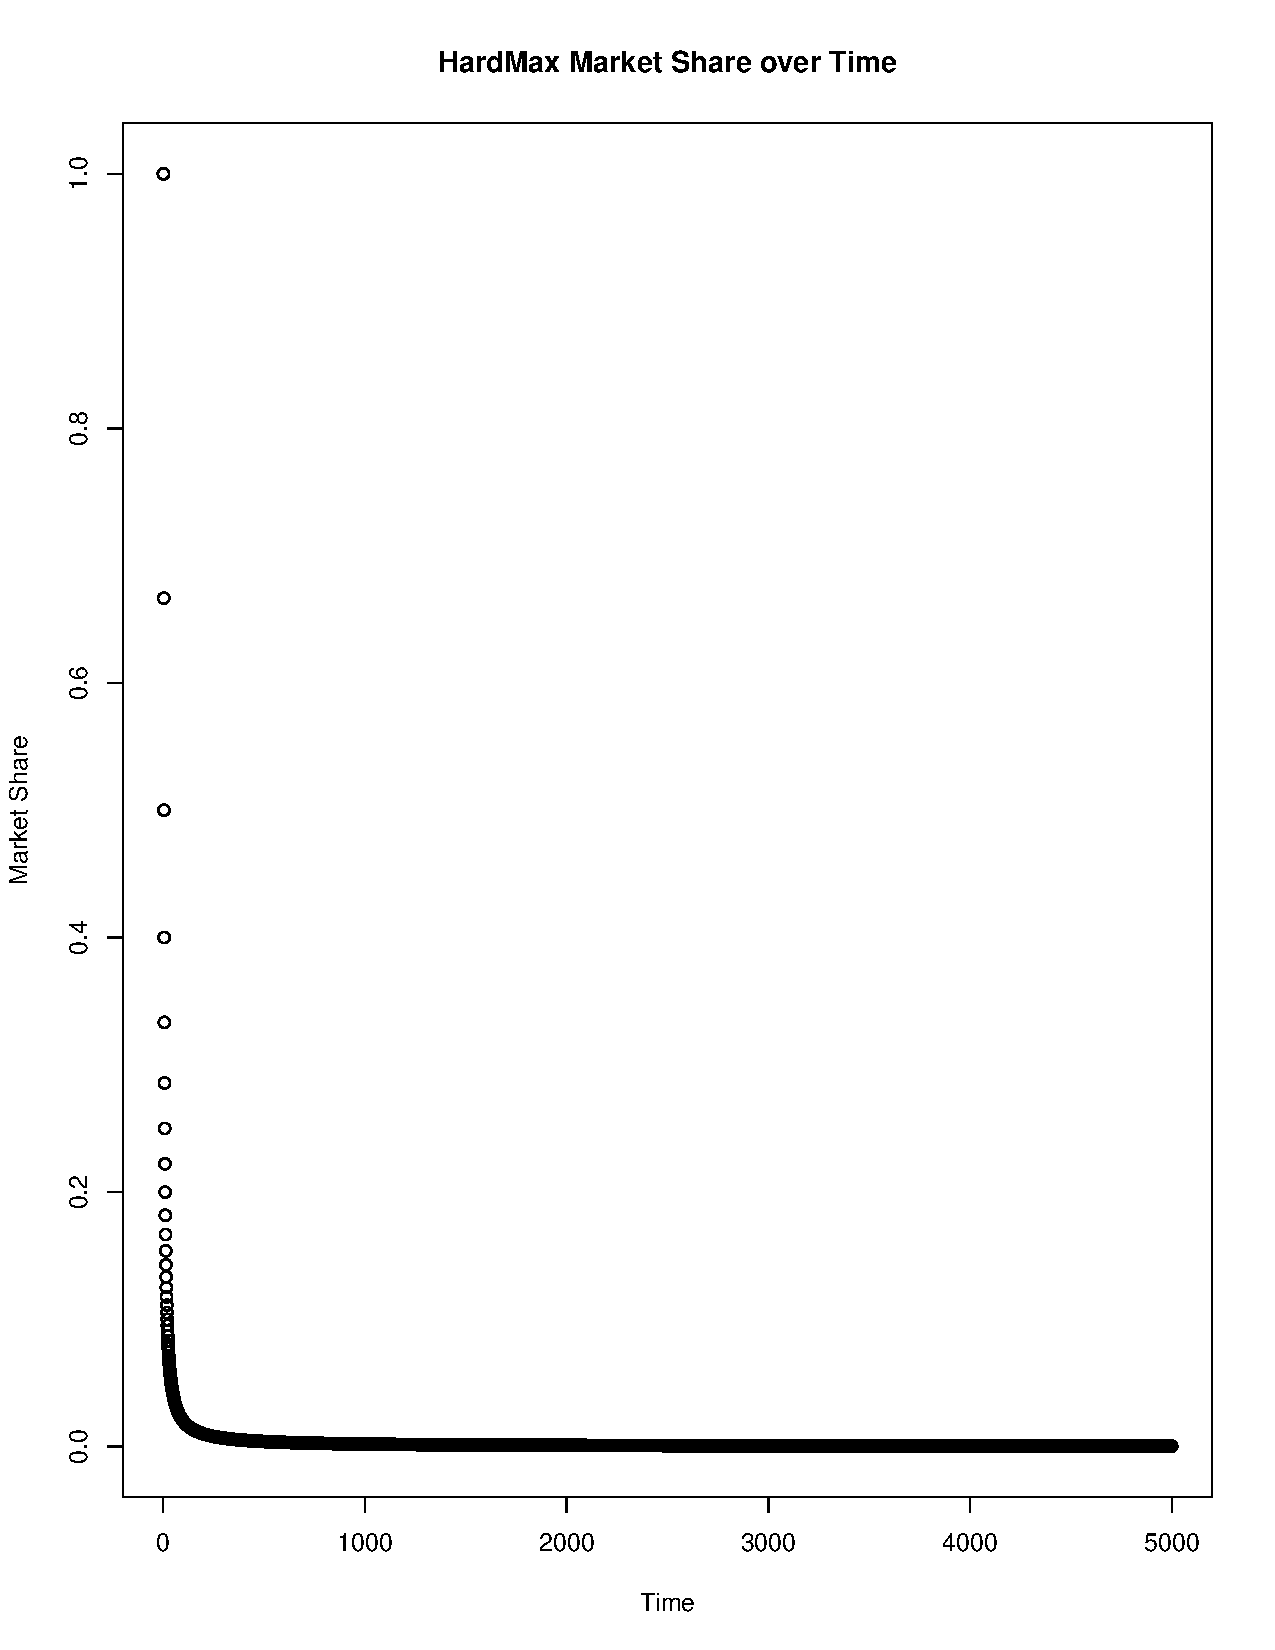
\includegraphics[scale=0.30]{decreasing_ms_over_time} \\
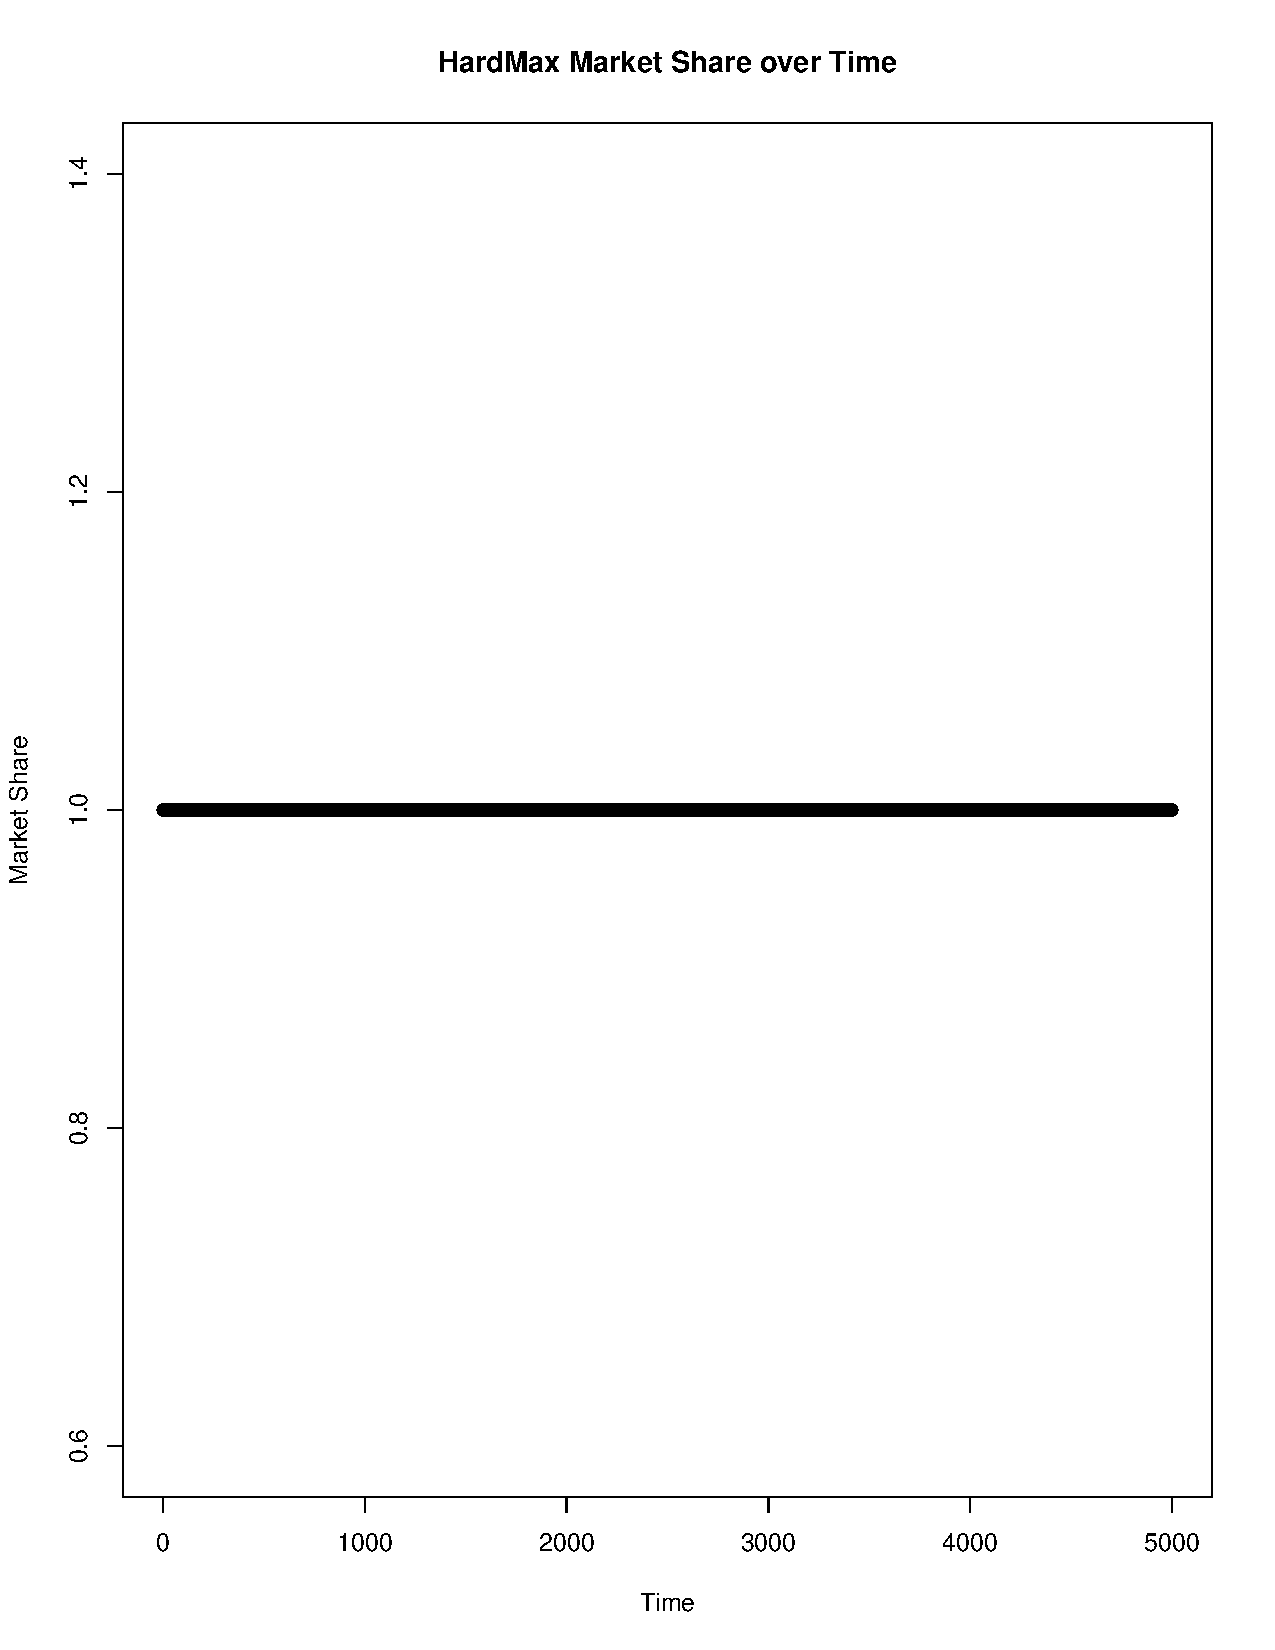
\includegraphics[scale=0.30]{standard_ms_over_time} \\
\vspace{0.25cm}

However, there are some simulations where we do not observe this. For instance, \\
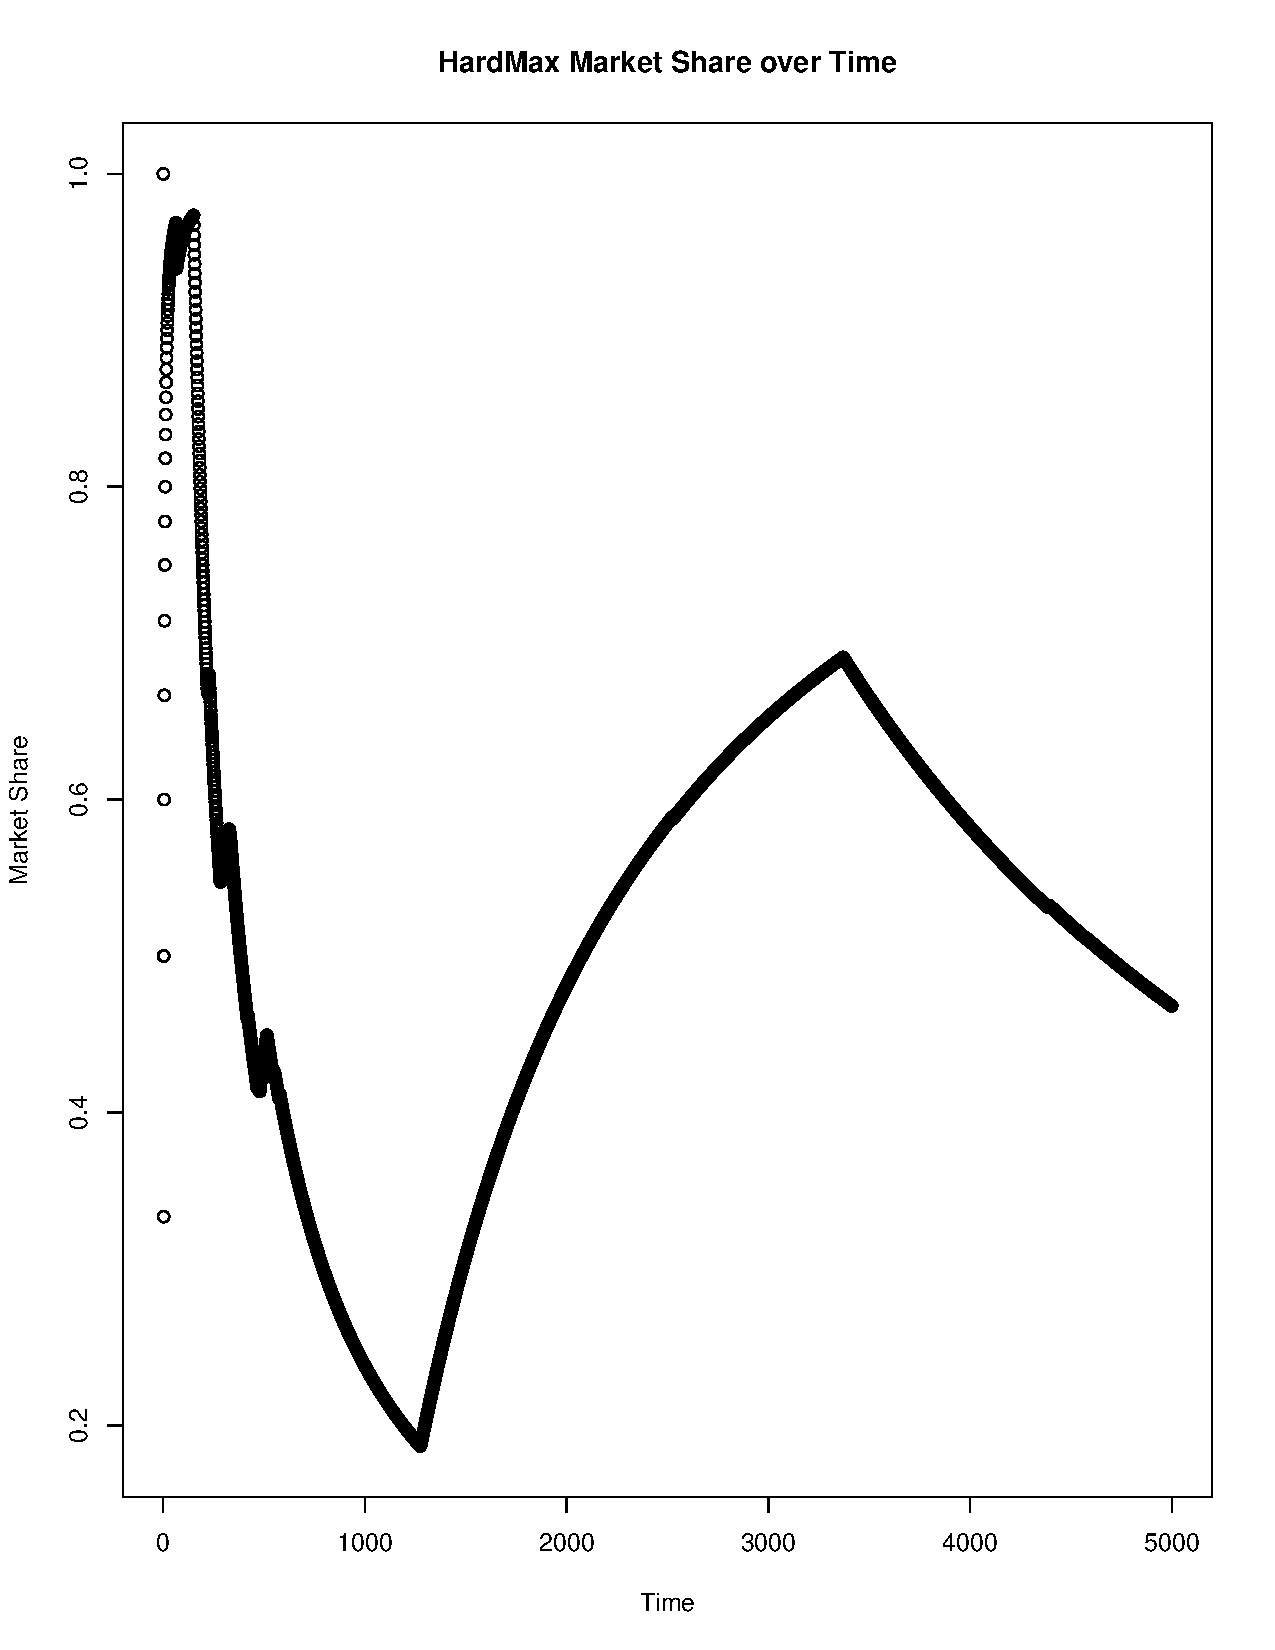
\includegraphics[scale=0.30]{odd_ms_over_time} \\

I am not sure what happens in these cases, but one conjecture is that these arise from random noise from a low memory size (memory here is 100, as we have been using in our experiment). I've re-run this experiment for a memory size of 1000 and there are fewer cases which have odd switches as shown above. However, would need to look into this more if we think this is worth digging into more. Another thing that might be interesting here is to ask what happens with HardMax if we get rid of any random noise in the reputation score and make it purely dependent on arm selection. In other words, what happens if the reputation score is constructed by using the true means of the selected arms. This of course is not a realistic model but may be useful for thinking about what is going on in this case. The results for this are reported in the appendix.\\

As a comparison, what do the trajectories for the HardMaxWithRandom agent response functions look like? Haven't dug too deeply into the data for these simulations, but here is a sample one (ThompsonSampling vs DEG - plotted market share is for ThompsonSampling) that is similar to many in those that I have looked at: \\
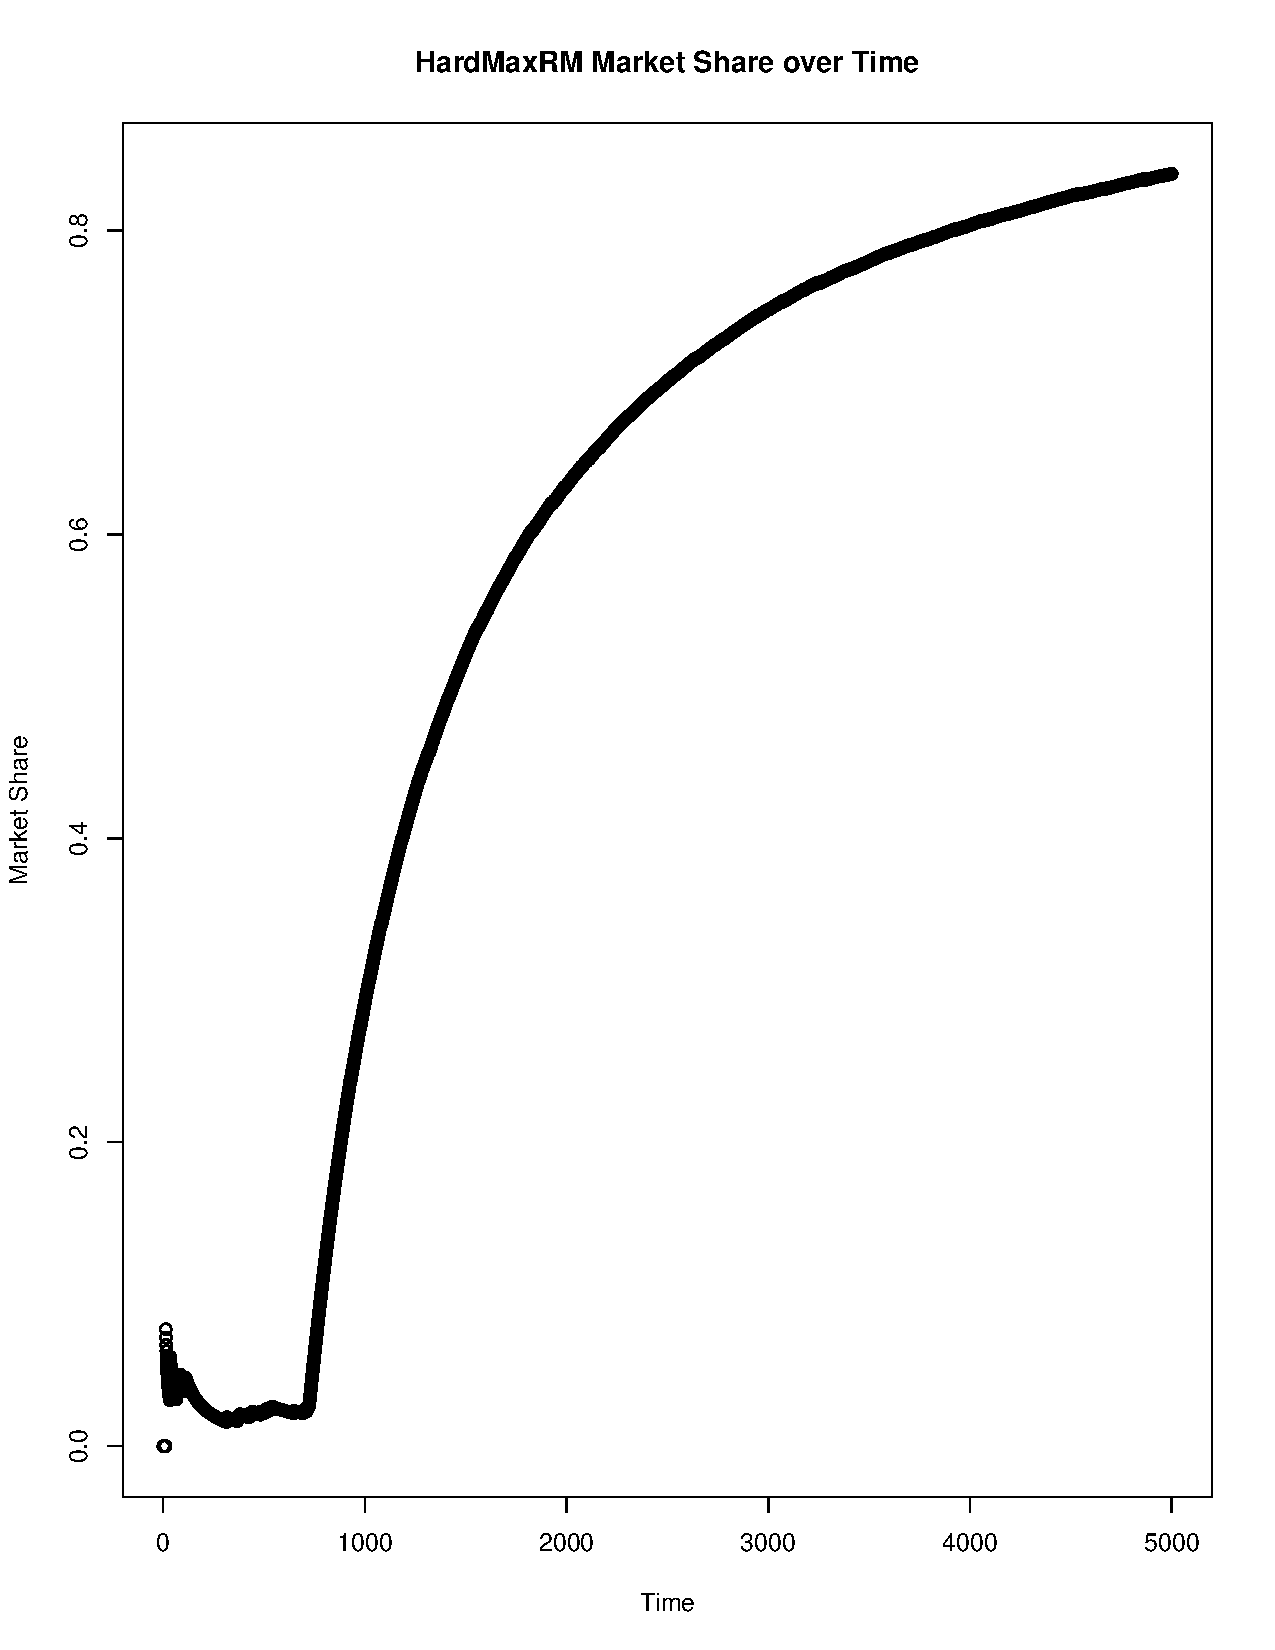
\includegraphics[scale=0.25]{hmr_over_time} \\
\textbf{Puzzles}: Inconsistent with this interpretation of the HardMax results is the result for the Heavy Tail prior. Why does Thompson Sampling do so poorly! Looking at the reputation plots we see that in the early rounds there is very little difference between the algorithms but Thompson Sampling still does better, even if only slightly. Thus, it's kind of confusing as to what is actually going on. Perhaps worth looking more closely at some of the trajectory plots for this prior. As well, Bayesian Greedy seems to beat Bayesian Epsilon Greedy on this prior even when there is randomness in the agent response model which seems puzzling given the preliminary plots. \\

In general, the conjecture that differences in algorithm performance in early rounds is important for determining results in HardMax and differences in algorithm performance for large $T$ is important for determining results in HardMaxWithRandom and SoftMax seems to be roughly validated (but there are some cases we need to think more about what is happening).

\section*{Incumbent Experiment}
Now, we change $X = 200$. In words, we give principal 2 $X$ free observations (the ``incumbent") and this updates her information set and reputation amongst the agents. In this setting what should the incumbent do? What should the entrant do? Does this depend on the agent model? I would conjecture that when we have sufficient randomness in the agent model the same conclusions as before should hold - namely that the entrant, even if getting beat upon entry, should eventually get enough ``free" observations that she can catch up and take more of the market. However, the time horizon, in contrast to the simultaneous entry case, seems like it may be way longer! So far, most of the simulations have simply looked at $t = 1000$, but it may make sense to look at longer time horizons due to the conjecture from above. \\
\vspace{0.25cm}

What about with HardMax? The only intuition I have is for the incumbent. For the entrant, it is not clear to me what the entrant should do. For the incumbent, in our simulations we fix a $X$ when the entrant will come in and the incumbent should want to maximize both the information that she accrues before then and the reputation that she amongst the agents. However, this seems exactly like the standard exploration exploitation dilemma where reputation is simply the cumulative reward and ``smart" algorithms like Thompson Sampling ought to be better than the ``dumb" algorithms at maximizing information gain while at the same time optimizing cumulative reward. Thus, I expect that Thompson Sampling should be in a better starting position at the start of the competing bandits game (we can view the incumbent experiment as being the simultaneous entry game where the incumbent starts with a head start in terms of information and reputation) and thus control more of the market. This seems to be the case in the reported simulations, both with large $X = 200$ and $X = 100$. Below are the result for $X = 200$ ($X = 100$ is in the appendix figures)

To read the tables: the columns represent the algorithm played by the incumbent and the row represents the algorithm played by the incumbent. For instance, looking at the second cell in the first row we have that the Incumbent played Dynamic (Bayesian) Epsilon Greedy and the entrant played Thompson Sampling and the reported mean is the average market share for the entrant.

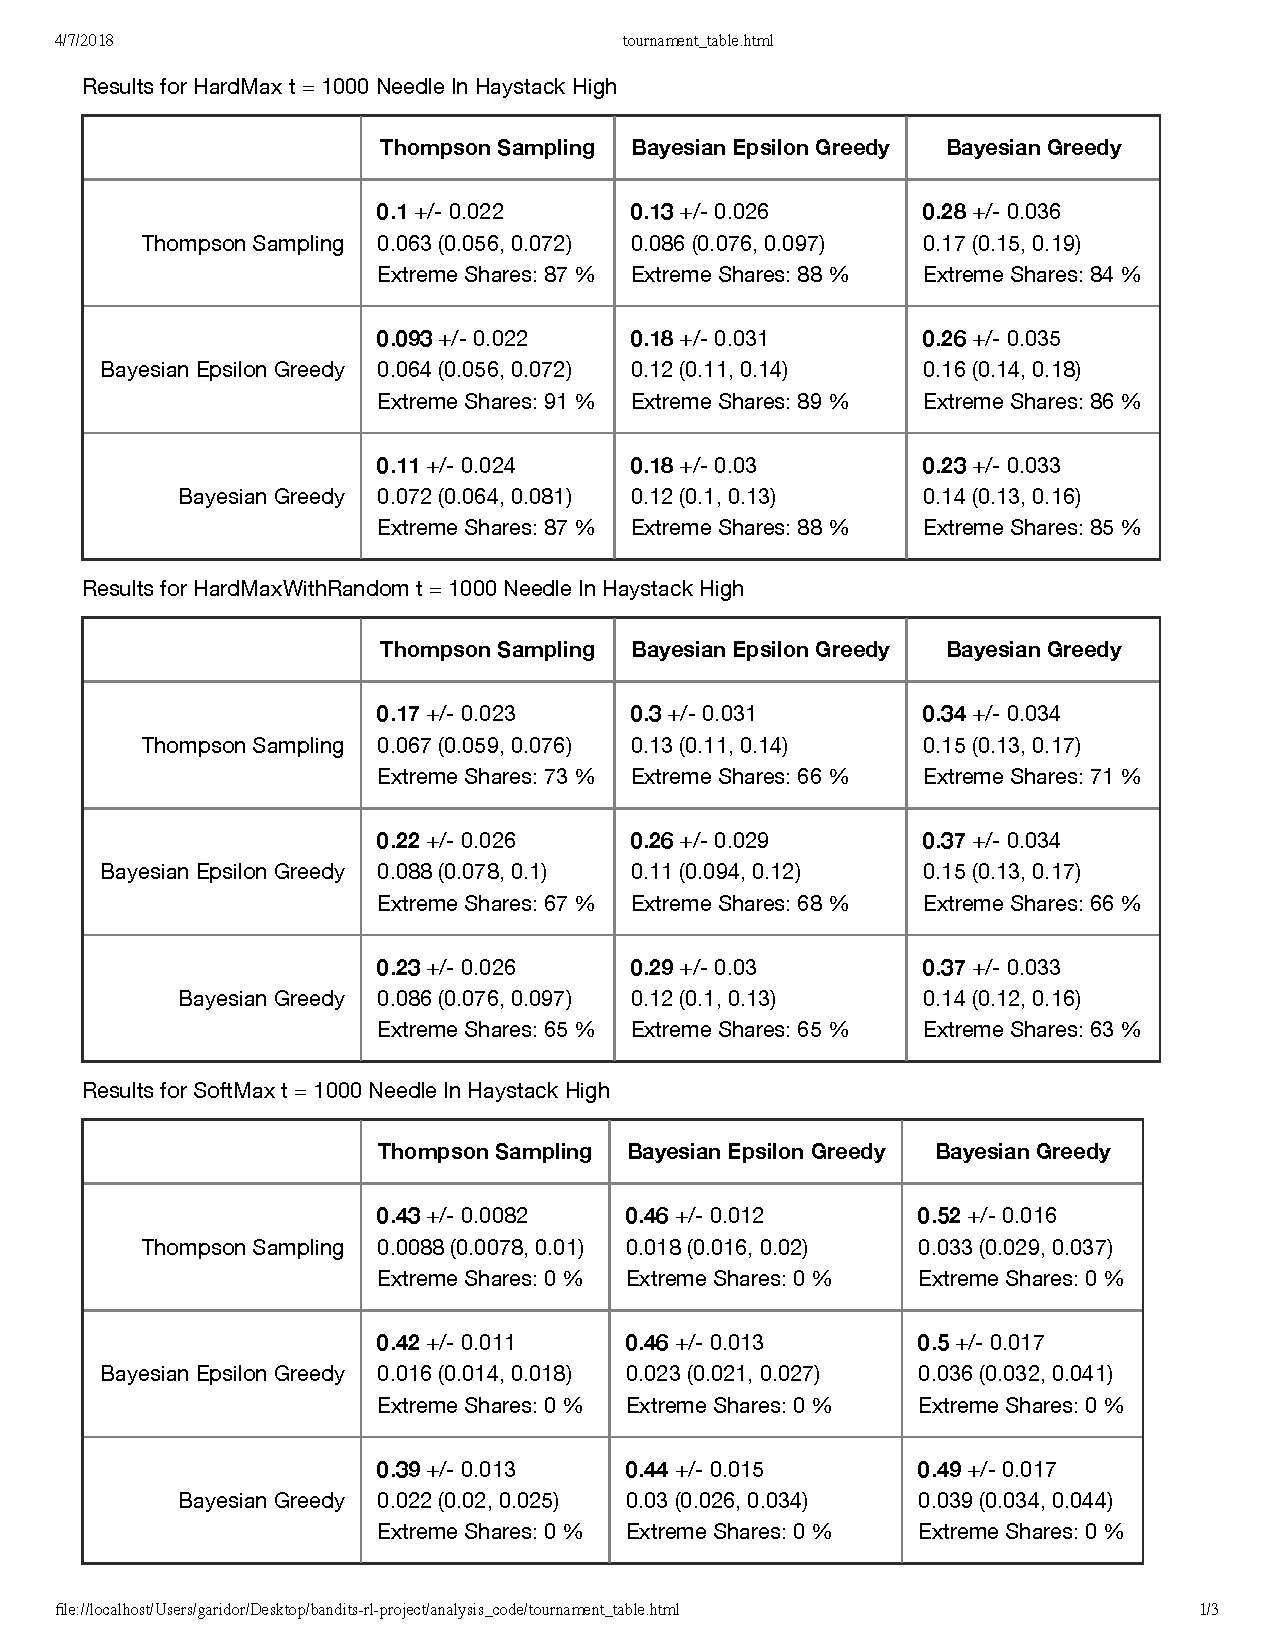
\includepdf[pages={-}]{free_obs_tournament}

What next? Have re-run this for lower values of $X$ and higher $T$ (3000) and seen qualitatively similar results. Some potential follow-up questions of interest are:
\begin{enumerate}
\item Does reputation or information play a bigger role in the dominance of the incumbent? Can test this by re-initializing either reputation or information of the incumbent when the entrant wins the market (and re-running simulations of that).
\item Even for HardMax it seems that the entrant gets a non-zero market share (the average seems to be between .05 and .25 usually). What do the market share trajectories look like? Are there a lot of simulations where the entrant simply gets zero and some where the entrant seems to get lucky upon entry and has an increasing market share over time?
\item Run for a larger time horizon for the models with agent randomness to see if better algorithms win in the long-run.
\end{enumerate}

\section*{Appendix}

This contains some figures which are useful, but seem second-order to me.

\subsection*{Preliminary Simulations}

The plots for the realized rewards for each of the priors:

\includegraphics[scale=0.5]{"../results/preliminary_figures/Instantaneous Realized Reward Trajectory for Needle In Haystack 1 High 3 arms"} \\
\includegraphics[scale=0.5]{"../results/preliminary_figures/Instantaneous Realized Reward Trajectory for Uniform 3 arms"} \\
\includegraphics[scale=0.5]{"../results/preliminary_figures/Instantaneous Realized Reward Trajectory for Heavy Tail 3 arms"}

\subsection*{Simultaneous Entry}

The following is the result of running simulations where instead of the realized reward being utilized to form the reputation score, the TRUE mean of the selected arm was included in the reputation score.\\
\includegraphics[scale=0.5]{"reputation_true_mean"}

\subsection*{Asymmetric Entry}

The following is the result of running the incumbent experiment with $X = 100$

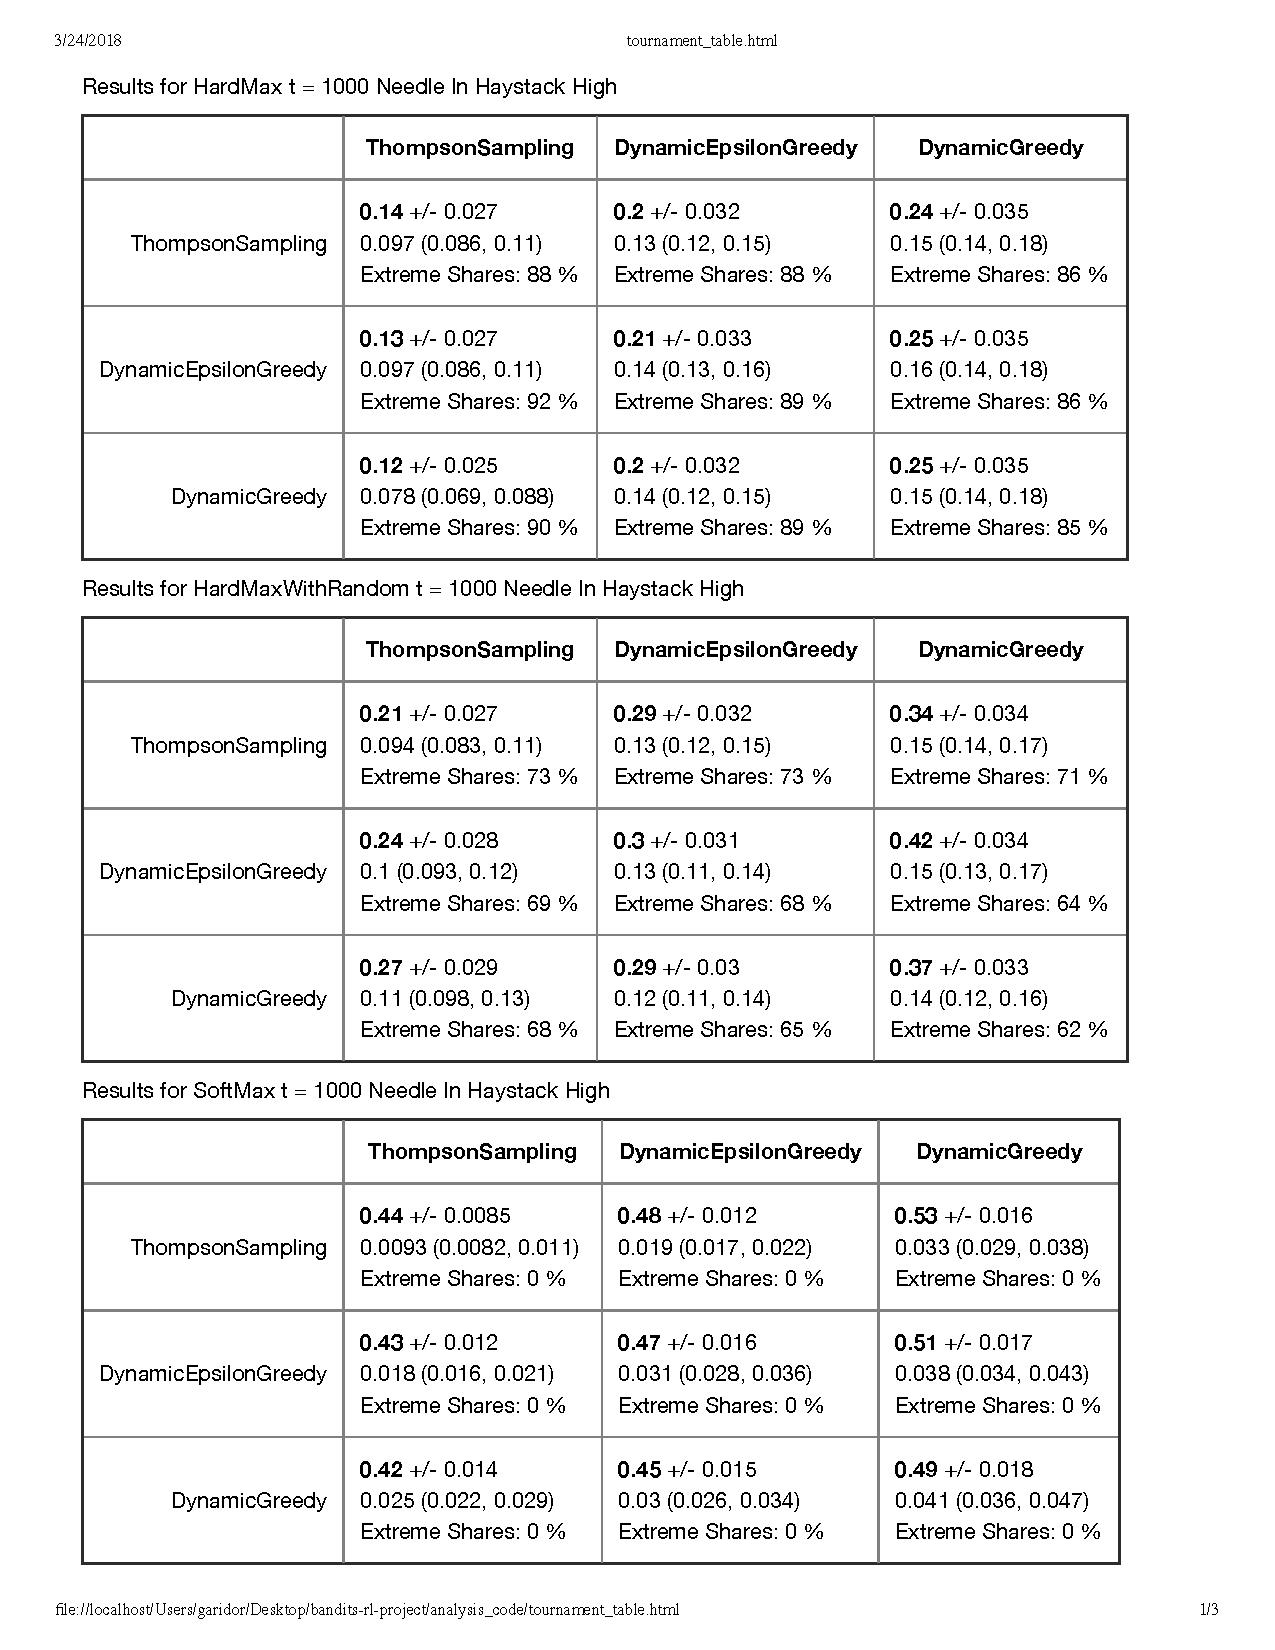
\includepdf[pages={-}]{less_free_obs_tournament_table}


\end{document}